% Compile from this folder with: sh build_report.sh
% All figures, numerical tables, and supporting result snapshots are bundled.
\documentclass[11pt,letterpaper]{article}
\usepackage[margin=0.85in,headheight=15pt]{geometry}
\usepackage[T1]{fontenc}
\usepackage[utf8]{inputenc}
\usepackage{lmodern,microtype}
\usepackage{amsmath,amssymb}
\usepackage{graphicx,booktabs,tabularx,array}
\usepackage[table]{xcolor}
\usepackage{caption,float,placeins}
\usepackage{enumitem,fancyhdr,titlesec}
\usepackage{tikz}
\usetikzlibrary{arrows.meta,positioning}
\usepackage{listings}
\usepackage{hyperref}

\definecolor{ink}{HTML}{163640}
\definecolor{teal}{HTML}{117C77}
\definecolor{pale}{HTML}{EDF5F3}
\definecolor{muted}{HTML}{53666D}
\definecolor{amber}{HTML}{B7602C}
\hypersetup{colorlinks=true,linkcolor=teal,citecolor=teal,urlcolor=teal,
  pdftitle={Parking-Lot Stormwater Detention: Engineering Project Report},
  pdfauthor={Prepared for Manasi; technical study and report developed with Codex},
  pdfsubject={Project idea, engineering goals, hydrology, storage routing, design comparison, and results}}
\titleformat{\section}{\Large\sffamily\bfseries\color{ink}}{\thesection}{0.7em}{}
\titleformat{\subsection}{\large\sffamily\bfseries\color{ink}}{\thesubsection}{0.7em}{}
\titleformat{\subsubsection}{\normalsize\sffamily\bfseries\color{ink}}{\thesubsubsection}{0.7em}{}
\titlespacing*{\section}{0pt}{19pt}{9pt}
\titlespacing*{\subsection}{0pt}{13pt}{6pt}
\setlength{\parindent}{0pt}
\setlength{\parskip}{6pt}
\setlength{\tabcolsep}{5pt}
\renewcommand{\arraystretch}{1.2}
\setlist{itemsep=3pt,topsep=4pt,leftmargin=1.4em}
\captionsetup{font=small,labelfont=bf,skip=7pt}
\pagestyle{fancy}
\fancyhf{}
\fancyhead[L]{\small\sffamily\color{ink}MANASI PROJECT \; / \; STORMWATER DETENTION}
\fancyhead[R]{\small\sffamily Engineering report}
\fancyfoot[L]{\footnotesize\color{muted}Conceptual simulation study \enspace\textbar\enspace September 2026}
\fancyfoot[R]{\small\thepage}
\renewcommand{\headrulewidth}{0.4pt}
\setcounter{tocdepth}{1}
\setcounter{secnumdepth}{2}
\setlength{\emergencystretch}{2em}
\newcommand{\mthree}{\ensuremath{\mathrm{m^3}}}
\newcommand{\file}[1]{\texttt{\detokenize{#1}}}
\newcommand{\source}[1]{\par\vspace{3pt}{\footnotesize\raggedright\color{muted}Source: #1\par}}
\newcolumntype{Y}{>{\raggedright\arraybackslash}X}
\lstset{basicstyle=\ttfamily\footnotesize,breaklines=true,
  frame=single,rulecolor=\color{teal!35},backgroundcolor=\color{pale},
  columns=fullflexible,keepspaces=true,showstringspaces=false}

\begin{document}
\hypersetup{pageanchor=false}
\begin{titlepage}
\thispagestyle{empty}
{\sffamily\color{teal}\bfseries ENGINEERING PROJECT REPORT\par}
\vspace{0.35in}
{\sffamily\bfseries\color{ink}\fontsize{29}{34}\selectfont
Parking-Lot\par Stormwater Detention\par}
\vspace{0.18in}
{\sffamily\Large\color{muted}From project idea to simulation,\par design selection, and engineering evaluation\par}
\vspace{0.28in}
{\large Prepared for Manasi\par}
{\color{muted}Project: \file{manasi_project}\par September 8, 2026\par}
\vspace{0.2in}
{\color{teal}\rule{\linewidth}{1.2pt}}

\vspace{0.12in}
{\sffamily\large\bfseries\color{ink}Abstract\par}
This project investigates how temporary storage can reduce the peak discharge
from a hypothetical parking lot while meeting explicit overflow and drainage
targets. The study models a 4,000 m$^2$ parking catchment and an adjacent
200 m$^2$ detention footprint. Nine synthetic one-hour storms combine rainfall
depths of 25, 50, and 100 mm with uniform, front-loaded, and back-loaded
distributions. Event runoff is calculated using cumulative curve-number
losses, transformed into an inflow hydrograph using a volume-normalized SCS
response, and routed through constant-area storage with an idealized square
outlet. An implicit numerical solution conserves water and explicitly records
overflow.

The design search evaluates 24 storage--outlet combinations against all nine
storms. The smallest tested design satisfying all three 50 mm storm shapes
provides 150 m$^3$ of storage at 0.75 m modeled depth with a
100 $\times$ 100 mm opening. Its peak reduction ranges from 63.09\% to
74.39\%, with zero overflow and a maximum drawdown time of 7.81 hours after
rainfall ends. Verification includes 16 passing numerical tests, water-balance
checks, and refinement of the complete grid to a 1.875 s time step.

The selected design overflows during the 100 mm storms and fails one
CN~100 sensitivity case. The findings therefore support a conditional
conceptual selection under the stated assumptions. The modeled benefit is
reduced peak flow and delayed discharge; detention does not remove the
incoming runoff volume.

\vspace{0.08in}
\colorbox{pale}{\parbox{\dimexpr\linewidth-2\fboxsep\relax}{%
\small\textbf{Selected nominal configuration}\quad
150 m$^3$ storage\; $\cdot$\; 200 m$^2$ footprint\; $\cdot$\; 0.75 m depth\\
100 $\times$ 100 mm opening\; $\cdot$\; minimum design-event peak reduction 63.09\%
}}
\vfill
{\footnotesize\color{muted}Report basis: the completed project run and saved
results dated September 8, 2026. Technical implementation and documentation
were developed with Codex. Manasi's individual review remains pending in the
project contribution record.}
\end{titlepage}

\pagenumbering{roman}
\hypersetup{pageanchor=true}
\tableofcontents
\vspace{0.25in}
\textbf{Reading guide.} Sections~\ref{sec:idea}--\ref{sec:basis} establish
the project idea and design objectives. Sections~\ref{sec:methods} and
\ref{sec:implementation} explain how the study was performed.
Sections~\ref{sec:results}--\ref{sec:sensitivity} present the measured
simulation outputs and their numerical checks. Section~\ref{sec:discussion}
interprets the design decision and its limits. The appendices provide the
complete candidate comparison and instructions for reproducing the work.

\textbf{Evidence convention.} Numerical results in this report come from the
saved project outputs, with copies in \file{source_data/}. Tables are generated
directly from those copies. The cited engineering manuals support the method;
the geometry, synthetic rainfall, parameter choices, and acceptance targets
are project assumptions. Values are rounded for presentation, while design
decisions use the saved full-precision values.
\clearpage
\pagenumbering{arabic}

\section{Project Idea and Engineering Goals}\label{sec:idea}
\subsection{Origin of the project}
The project began with a practical engineering question: can a compact
detention facility temporarily store parking-lot runoff and release it slowly
enough to reduce the downstream peak? The supplied project plan framed this
as a manageable study connecting fluid mechanics, numerical methods, Python
analysis, spreadsheet checks, and conceptual drafting.\cite{project_plan}
Its purpose was to develop an engineering argument from stated assumptions
through calculations and comparison to a defensible design choice.

A parking lot provides a simple catchment with a high assumed runoff
response. During a storm, runoff can arrive faster than a restricted outlet
can release it. A detention basin accommodates the difference as stored
water. Water depth then controls discharge through the opening. The resulting
tradeoff is central to the project: a smaller opening can suppress controlled
flow but may increase storage requirements, overflow, and drainage time.
Capacity and outlet size must therefore be evaluated together.

The study uses a hypothetical site so the modeling assumptions can be
examined explicitly and reproduced without field data. Its results describe
the behavior of that conceptual system. No measured flooding history,
surveyed drainage pattern, or location-specific storm frequency was supplied.

\subsection{Primary question and acceptance criteria}
The primary question is:
\begin{quote}
What is the smallest tested storage capacity that reduces the peak downstream
discharge by at least 50\%, avoids overflow, and drains below 1\% of capacity
within 24 hours after the selected storm ends?
\end{quote}
The design event is 50 mm of rain in 60 minutes. A candidate must meet every
criterion for \emph{each} of the three temporal storm shapes. The criteria
are educational targets fixed before comparison, rather than adopted local
drainage requirements.

\begin{table}[H]
\centering\small
\caption{Project objectives and the quantities used to assess them.}
\begin{tabularx}{\linewidth}{p{0.23\linewidth}Y}
\toprule
Objective & Assessment rule \\
\midrule
Peak attenuation & At least 50\% reduction relative to the matching baseline;
downstream flow includes controlled discharge and overflow. \\
Overflow avoidance & Total overflow no greater than $10^{-6}$ m$^3$, the
specified numerical tolerance. \\
Drainage recovery & Final crossing below 1\% of nominal capacity within 24 h
after rain ends, with no later rebound above the threshold. \\
Storage economy & Choose the lowest-capacity passing option in the tested grid. \\
Reliable computation & Check water balance, limiting cases, and time-step
refinement before interpreting the result. \\
\bottomrule
\end{tabularx}
\end{table}

Secondary goals are to explain why alternatives fail, examine performance
at 25 and 100 mm rainfall, test selected assumptions, and produce a reproducible
set of calculations, figures, and engineering deliverables. Cost, land value,
and construction quantities are not included in the optimization objective.

\section{Site Concept and Design Basis}\label{sec:basis}
\subsection{Geometry and a consistent baseline}
The parking catchment measures 80 $\times$ 50 m, giving a contributing area
$A_p=4{,}000$ m$^2$. The adjacent basin footprint measures 20 $\times$ 10 m,
giving a fixed area $A_b=200$ m$^2$. The total study area is therefore
4,200 m$^2$ for both the baseline and detention alternatives.

In the baseline, the reserved basin footprint is represented as an impervious
collection pad with negligible storage and loss. Its rainfall passes directly
to the downstream comparison point. In a detention alternative, rainfall on
that same footprint enters storage together with parking runoff. This keeps
the contributing area and prescribed event input volume consistent. Omitting
the footprint from the baseline would change the comparison itself.

\begin{table}[H]
\centering\small
\caption{Nominal inputs and the design search space.}\label{tab:inputs}
\begin{tabularx}{\linewidth}{p{0.37\linewidth}Y}
\toprule
Quantity & Adopted value \\
\midrule
Parking area; basin footprint & 4,000 m$^2$; 200 m$^2$ \\
Curve number; initial abstraction & CN = 98; $I_a=0.2S$ \\
Catchment lag & 10 min \\
Storm depths and duration & 25, 50, 100 mm; 60 min for each event \\
Storm distributions & Uniform, front-loaded, back-loaded; six 10-min blocks \\
Candidate depths & 0.15, 0.30, 0.45, 0.60, 0.75, 0.90 m \\
Candidate storage capacities & 30, 60, 90, 120, 150, 180 m$^3$ \\
Square opening side lengths & 40, 60, 80, 100 mm \\
Outlet coefficient and gravity & $C_d=0.62$; $g=9.80665$ m/s$^2$ \\
Initial basin storage & 0 m$^3$ at the start of each independent event \\
Basin infiltration; evaporation & Both zero \\
Time step & Initially 30 s; final accepted step 1.875 s \\
Simulation horizon & Initially 30 h; extend by doubling if required,
up to the configured 240 h cap \\
\bottomrule
\end{tabularx}
\source{Bundled \file{source_data/config_used.json}.}
\end{table}

The basin follows a constant-area stage--storage relationship,
$V=A_bh$. Thus, an increase in modeled depth increases capacity without
changing the footprint. Vertical boundaries in the drawing illustrate this
accounting geometry; the study does not size structural walls or prescribe
an excavated basin with safe side slopes.

\clearpage
\subsection{Scope of the engineering representation}
The system contains one lumped parking catchment, one inflow hydrograph,
one level-pool storage element, and one freely discharging control opening.
The adopted CN, lag, and discharge coefficient are preliminary assumptions.
The storms have no assigned recurrence intervals. Tailwater, pipe friction,
debris blockage during the design events, water-quality treatment, groundwater,
and sequences of storms with incomplete recovery are not modeled.

These choices isolate the interaction between rainfall timing, runoff,
storage, and outlet discharge. They also define the practical boundary of the
finding: a passing simulated configuration is a conceptual candidate for
further development, rather than a completed site drainage design.

\begin{figure}[H]
\centering
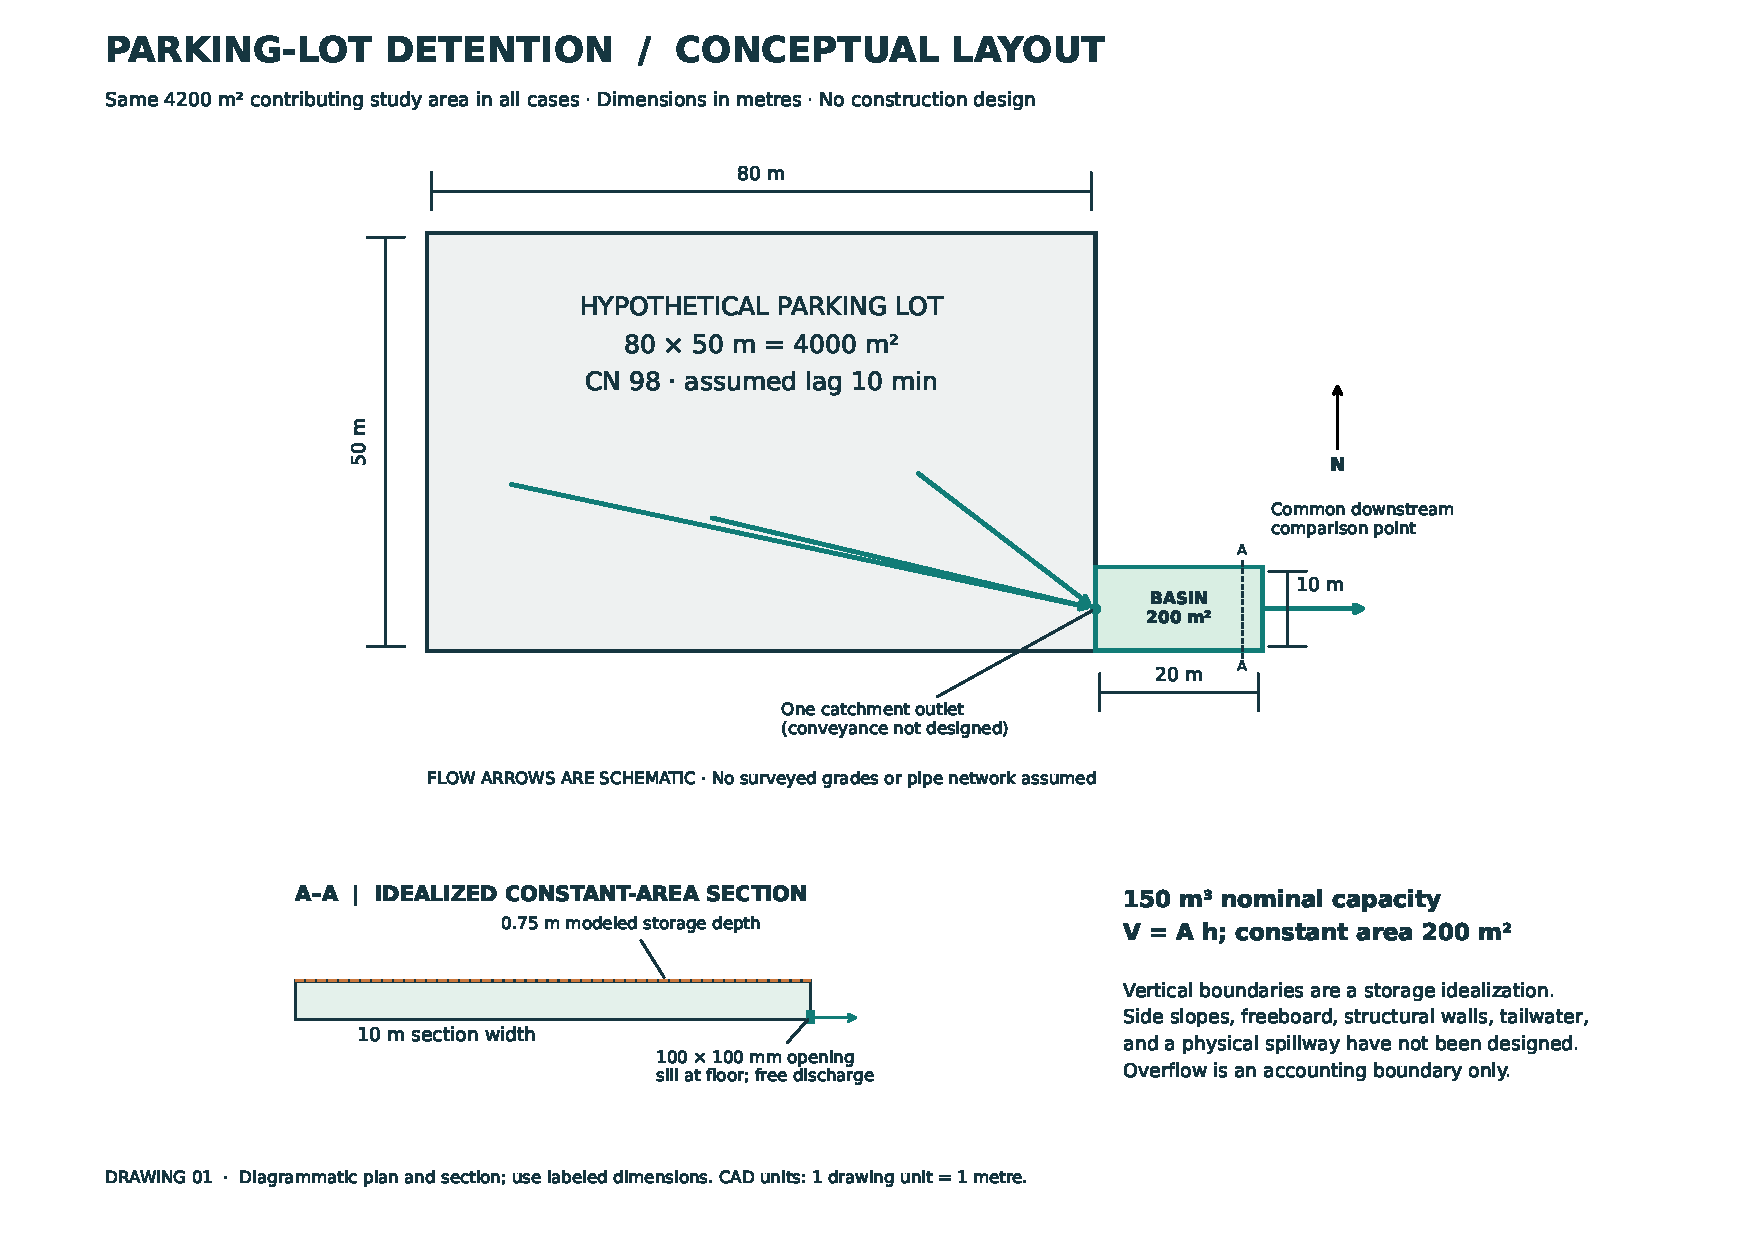
\includegraphics[width=\linewidth]{figures/site_plan.pdf}
\caption{Conceptual site plan and basin section from the completed project.
The labeled dimensions define the hypothetical geometry. Flow arrows are
schematic; surveyed grades, conveyance, freeboard, and a physical spillway
are outside the model.}\label{fig:site}
\end{figure}

\clearpage
\section{Engineering Methods}\label{sec:methods}
\subsection{Rainfall construction}
Each one-hour event contains six equal ten-minute blocks. For total rainfall
$P_{\mathrm{tot}}$ and relative block weights $r_k$, block depth is
\begin{equation}
 P_k=P_{\mathrm{tot}}\frac{r_k}{\sum_{j=1}^{6}r_j}.
 \label{eq:rain}
\end{equation}
The vectors are $(1,1,1,1,1,1)$ for uniform rainfall,
$(6,5,4,3,2,1)$ for front-loaded rainfall, and
$(1,2,3,4,5,6)$ for back-loaded rainfall. For the 50 mm event, uniform
intensity is 50 mm/h throughout the hour. The front-loaded intensities are
approximately 85.71, 71.43, 57.14, 42.86, 28.57, and 14.29 mm/h; the
back-loaded sequence reverses that order.

The implementation integrates the constant-intensity blocks over each
computational interval, including intervals that cross a block boundary.
It verifies that rainfall increments sum to the specified event depth.
Storm shapes change the timing of rainfall while preserving total depth
and duration.

\subsection{Cumulative runoff losses}
The NRCS/SCS curve-number method calculates cumulative excess rainfall from
cumulative precipitation. With $P$, $S$, $I_a$, and $P_e$ in millimetres,
\begin{align}
 S &= \frac{25400}{\mathrm{CN}}-254, & I_a&=0.2S,\label{eq:retention}\\
 P_e(P)&=
 \begin{cases}
 0, & P\leq I_a,\\[2pt]
 \displaystyle\frac{(P-I_a)^2}{P-I_a+S}, & P>I_a.
 \end{cases}\label{eq:cn}
\end{align}
These equations and the event-based interpretation follow the USACE
description of the SCS CN loss model.\cite{cn}
For an interval bounded by $t_n$ and $t_{n+1}$, the runoff depth is
\begin{equation}
 \Delta P_{e,n}=P_e(P(t_{n+1}))-P_e(P(t_n)),\qquad
 v_{p,n}=\frac{A_p\Delta P_{e,n}}{1000}.
 \label{eq:excess}
\end{equation}
Here $v_{p,n}$ is generated parking-runoff volume in m$^3$. Initial abstraction
is applied once through the cumulative event calculation; it is not restarted
at every interval. The event state resets between independent storms.
CN~100 is handled explicitly as $P_e=P$, including at zero rainfall. The
parking area receives no additional impervious-area multiplier.

For the nominal 50 mm event, the worked calculation is
\begin{align*}
 S &= 5.183673\ \mathrm{mm}, & I_a&=1.036735\ \mathrm{mm},\\
 P_e &=44.275843\ \mathrm{mm}, &
 V_{\mathrm{parking}}&=177.103371\ \mathrm{m^3}.
\end{align*}
Direct rainfall on the basin footprint adds
$200(50/1000)=10.000000$ m$^3$, so total input to either alternative is
187.103371 m$^3$. This scalar check supplies an independent reference for the
time-series water balance.

\subsection{Runoff hydrograph transformation}
Detention routing needs the time history of inflow as well as its total
volume. A peak-only estimate cannot resolve temporary storage through the
event. TxDOT's runoff-method guidance identifies hydrograph methods for
storage applications.\cite{method_selection}

The project uses the 33 dimensionless SCS/NRCS hydrograph ordinates in TxDOT
Table~4-29, stored locally as \file{scs_dimensionless_uh.csv}.\cite{ordinates}
For each excess-rainfall interval, the response time to peak is
\begin{equation}
 T_p=t_{\mathrm{lag}}+\frac{\Delta t}{2},
 \label{eq:tp}
\end{equation}
measured from the beginning of the pulse. This follows the SCS
unit-hydrograph timing convention.\cite{uh}

The implementation linearly interpolates the dimensionless response
$f(t/T_p)$ and integrates it over each output interval. It converts these
integrals to nonnegative volume fractions $w_j$ satisfying
\begin{equation}
 w_j=\frac{\displaystyle\int_{j\Delta t}^{(j+1)\Delta t}f(t/T_p)\,dt}
 {\displaystyle\int_0^{5T_p}f(t/T_p)\,dt},\qquad \sum_j w_j=1,
 \label{eq:weights}
\end{equation}
where $f$ is zero beyond the reference tail. The transformed parking inflow is
the discrete convolution
\begin{equation}
 I_{p,n}=\sum_j v_{p,n-j}w_j.
 \label{eq:convolution}
\end{equation}
The complete response through $5T_p$ is retained. Normalization makes the
integrated parking hydrograph equal the generated parking-runoff volume.
The tabulated dimensionless discharge values are used as a response shape,
rather than interpreted directly as dimensional flow.

Direct footprint rainfall enters without this catchment-lag transformation.
For rainfall increment $\Delta P_n$, interval input and baseline flow are
\begin{equation}
 I_n=I_{p,n}+\frac{A_b\Delta P_n}{1000},\qquad
 Q_{b,n}=\frac{I_n}{\Delta t}.
 \label{eq:baseline}
\end{equation}
Here $I_n$ is a volume in m$^3$, while $Q_{b,n}$ is an interval-average
baseline flow in m$^3$/s.

\subsection{Storage and outlet hydraulics}
For fixed basin area, water depth is $h=V/A_b$. The opening is a vertical
square with side $a$, with its sill at the basin floor. Under the project's
free-discharge idealization, local velocity depends on the water head above
each wetted strip of the opening. Integrating across the wetted height gives
\begin{align}
 Q_c(h)&=\int_0^{\min(h,a)} C_d a\sqrt{2g(h-z)}\,dz\nonumber\\
 &=\frac{2}{3}C_d a\sqrt{2g}
 \left[h^{3/2}-\max(h-a,0)^{3/2}\right].
 \label{eq:outlet}
\end{align}
All lengths in this equation are in metres and discharge is in m$^3$/s.
The expression approaches zero continuously at an empty basin and accounts
for an opening that is only partly wetted at shallow depth.

For water well above the opening, the conventional centroid-head estimate
$Q_c\approx C_d a^2\sqrt{2g(h-a/2)}$ provides a useful independent comparison.
USACE documentation distinguishes outlet flow regimes and the limits of
submerged-orifice equations.\cite{outlet}
Equation~\eqref{eq:outlet} is the project's assumed rating, with constant
$C_d=0.62$; it is not a field-calibrated outlet or an assertion of equivalence
to a particular HEC-HMS structure model.

\subsection{Implicit storage routing and overflow accounting}
The governing conservation equation is
\begin{equation}
 \frac{dV}{dt}=Q_{\mathrm{in}}-Q_c-Q_o,
 \label{eq:continuity}
\end{equation}
where $Q_o$ is overflow discharge. The level-pool conservation concept follows
reservoir-routing practice.\cite{routing} The code uses a backward-Euler
storage step, whereas the cited HEC-HMS discussion describes a trapezoidal
Modified Puls formulation.

For a nonoverflowing interval, the next storage value satisfies
\begin{equation}
 V_{n+1}+\Delta t\,Q_c(V_{n+1}/A_b)=V_n+I_n.
 \label{eq:implicit}
\end{equation}
The code solves this scalar equation with SciPy's bracketed Brent solver
on $[0,\min(V_{\max},V_n+I_n)]$. The left side increases with storage, so
the bracket contains a unique physical solution when capacity is sufficient.
The controlled discharge assigned to the interval is the endpoint rating
$Q_c(V_{n+1}/A_b)$, whose product with $\Delta t$ supplies the step's
numerical discharge volume.

Let $W_n=V_n+I_n$ and $Q_{\mathrm{cap}}=Q_c(V_{\max}/A_b)$. If
$W_n\geq V_{\max}+\Delta t Q_{\mathrm{cap}}$, the update becomes
\begin{equation}
 V_{n+1}=V_{\max},\quad Q_{c,n}=Q_{\mathrm{cap}},\quad
 Q_{o,n}=\max\!\left(\frac{W_n-V_{\max}}{\Delta t}-Q_{\mathrm{cap}},0\right).
 \label{eq:overflow}
\end{equation}
Excess water is consequently retained in the accounting as overflow to the
same downstream point. It is not discarded by clipping the storage series.
The downstream discharge used in every comparison is
$Q_{d,n}=Q_{c,n}+Q_{o,n}$. Overflow is a capacity boundary calculation; no
spillway geometry or inundation hydraulics is represented.

\subsection{Performance metrics and numerical conventions}
Peak attenuation is calculated as
\begin{equation}
 R_Q=100\left(1-\frac{\max_n Q_{d,n}}{\max_n Q_{b,n}}\right).
 \label{eq:reduction}
\end{equation}
Each comparison uses the baseline generated with the same storm and catchment
parameters. Maximum depth follows from maximum storage divided by $A_b$.
The model also records overflow volume, discharge volume, residual storage,
time to peak, and drainage time.

Flows use interval values with midpoint timestamps; storage uses interval
boundaries. Therefore, flow volume is obtained by summing flow times
$\Delta t$, rather than trapezoidal integration of midpoint samples. Overflow
onset is recorded at the start of its first nonzero interval.

Drawdown is the elapsed time from rainfall end to the final interpolated
crossing below $0.01V_{\max}$, after which storage remains below that threshold.
For the selected capacity, this is 1.50 m$^3$, equivalent to 7.50 mm depth.
Exact emptying is not required: at shallow depth,
Equation~\eqref{eq:outlet} has $Q_c\propto h^{3/2}$, producing an asymptotic
recession. Any storage still present at the reporting horizon is included in
the water balance.

\clearpage
\section{Implementation and Experimental Workflow}\label{sec:implementation}
\subsection{Computational organization}
The project is implemented as a local Python workflow. Inputs are separate
from the hydrology, routing, comparison, and reporting modules, allowing an
assumption to be changed without rewriting the physical model.

\begin{figure}[H]
\centering
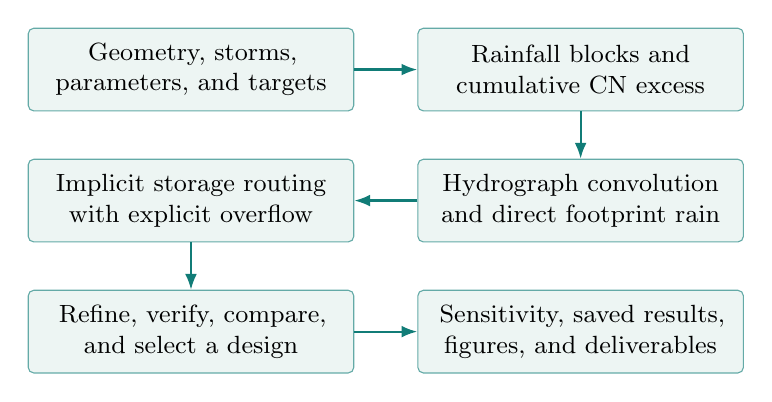
\begin{tikzpicture}[
 block/.style={draw=teal!65,fill=pale,rounded corners=2pt,align=center,
 font=\small,text width=3.9cm,minimum height=1.05cm},
 flow/.style={-{Latex[length=2mm]},thick,teal},node distance=0.6cm and 0.8cm]
\node[block] (inputs) {Geometry, storms,\\parameters, and targets};
\node[block,right=of inputs] (rain) {Rainfall blocks and\\cumulative CN excess};
\node[block,below=of rain] (uh) {Hydrograph convolution\\and direct footprint rain};
\node[block,left=of uh] (route) {Implicit storage routing\\with explicit overflow};
\node[block,below=of route] (check) {Refine, verify, compare,\\and select a design};
\node[block,right=of check] (output) {Sensitivity, saved results,\\figures, and deliverables};
\draw[flow] (inputs)--(rain);
\draw[flow] (rain)--(uh);
\draw[flow] (uh)--(route);
\draw[flow] (route)--(check);
\draw[flow] (check)--(output);
\end{tikzpicture}
\caption{Implemented engineering workflow. All numerical storm inputs and
reference hydrograph ordinates are available locally.}\label{fig:workflow}
\end{figure}

\begin{table}[H]
\centering\small
\caption{Main source modules and their responsibilities.}
\begin{tabularx}{\linewidth}{p{0.40\linewidth}Y}
\toprule
Source file & Responsibility \\
\midrule
\file{run_project.py} & Validate inputs, run tests and refinement, orchestrate
analysis and deliverable generation. \\
\file{stormwater/hydrology.py} & Rainfall increments, cumulative CN runoff,
unit-hydrograph weights, and baseline events. \\
\file{stormwater/routing.py} & Outlet rating, implicit storage solution,
overflow, and final drainage crossing. \\
\file{stormwater/study.py} & Scenario metrics, design selection, convergence
comparison, sensitivity, and independent checks. \\
\file{stormwater/figures.py} & Scientific plots and conceptual site drawings. \\
\file{stormwater/workbook.py} & Workbook tables, independent formulas,
checks, and charts. \\
\file{stormwater/dashboard.py} & Offline interactive scenario exploration. \\
\file{tests/test_model.py} & Hydrologic and hydraulic numerical tests. \\
\bottomrule
\end{tabularx}
\end{table}

\subsection{Design sweep and fixed selection rule}
Six capacities and four square opening sizes give 24 candidate designs.
Three rainfall depths and three storm shapes give nine events. Each design
is run against each event, giving $24\times9=216$ routed cases, plus nine
matching baselines at each time resolution.

Selection considers only the three 50 mm events. A design is feasible when
all three shapes satisfy peak reduction, overflow, and drawdown requirements.
Feasible designs are ranked first by increasing storage capacity, then by
shortest worst-case drawdown, least worst-case overflow, and finally largest
opening. This fixed order makes the decision reproducible and avoids selecting
an attractive hydrograph while overlooking a failing constraint.

The complete grid is repeated at successively halved time steps. The run
requires at least three resolutions, checks relative changes in downstream
peak, baseline peak, and maximum storage, and continues refinement until the
1\% target and decision-stability checks are met. The initial 30 h horizon
is extended when drainage has not been established; the longest horizon
needed in the completed core study was 60 h.

\subsection{Sensitivity experiment}
After selection, the chosen capacity and opening are held fixed. The model
varies CN through 95, 98, and 100; lag through 5, 10, and 15 min; and $C_d$
through 0.50, 0.62, and 0.75. Each value is run for all three 50 mm storm
shapes, giving 27 rows, including nominal repeats. Each comparison recomputes
its matching baseline. These are one-at-a-time experiments, rather than joint
worst-case combinations or measured parameter uncertainty distributions.

\section{Results}\label{sec:results}
\subsection{Runoff volume and baseline response}
At a fixed CN, storm shapes with the same total rainfall have the same
calculated runoff volume. Their flow peaks differ because the temporal
distribution and hydrograph response differ.
\begin{table}[H]
\centering\small
\caption{Event water inputs at nominal CN~98, common to every storm shape
and detention capacity for a given rainfall depth.}\label{tab:volumes}
% Generated by generate_tables.py from source_data/.
\begin{tabular}{rrrrr}
\toprule
\shortstack{Rainfall\\(mm)} & \shortstack{Parking excess\\(mm)} & \shortstack{Parking runoff\\(m$^3$)} & \shortstack{Direct rain\\(m$^3$)} & \shortstack{Total input\\(m$^3$)} \\
\midrule
25 & 19.701 & 78.806 & 5.000 & 83.806 \\
50 & 44.276 & 177.103 & 10.000 & 187.103 \\
100 & 94.038 & 376.150 & 20.000 & 396.150 \\
\bottomrule
\end{tabular}

\source{Bundled \file{source_data/baselines.csv}.}
\end{table}
For the design event, the baseline peak is 57.48 L/s for uniform rainfall,
73.19 L/s for front-loaded rainfall, and 85.67 L/s for back-loaded rainfall.
The highest baseline peak therefore occurs in the back-loaded case even
though all three events deliver the same 187.103 m$^3$ to the system.

\subsection{Selected capacity and outlet}
The smallest tested feasible design is \textbf{150 m$^3$ of nominal storage
at 0.75 m depth over 200 m$^2$, with a 100 $\times$ 100 mm opening}.
Table~\ref{tab:design_results} reports its performance for the three design
storm shapes.

\begin{table}[H]
\centering\small
\caption{Selected-design performance for the 50 mm storms. Drawdown is
measured after rainfall ends.}\label{tab:design_results}
% Generated by generate_tables.py from source_data/.
\begin{tabular}{lrrrrrr}
\toprule
Shape & \shortstack{Baseline\\(L/s)} & \shortstack{Detained\\(L/s)} & \shortstack{Reduction\\(\%)} & \shortstack{Max. storage\\(m$^3$)} & \shortstack{Overflow\\(m$^3$)} & \shortstack{Drawdown\\(h)} \\
\midrule
Uniform & 57.48 & 21.22 & 63.09 & 129.48 & 0.000 & 7.65 \\
Front-loaded & 73.19 & 21.04 & 71.25 & 127.55 & 0.000 & 7.51 \\
Back-loaded & 85.67 & 21.94 & 74.39 & 137.76 & 0.000 & 7.81 \\
\bottomrule
\end{tabular}

\source{Bundled \file{source_data/scenarios.csv}, design
\file{h0.750_o100}, final time step 1.875 s.}
\end{table}

The controlling storm depends on the metric. Uniform rainfall gives the
\emph{lowest percentage peak reduction}, 63.09\%, because its baseline peak
is lower. Back-loaded rainfall gives the \emph{greatest absolute detained
peak and storage demand}, 21.94 L/s and 137.761 m$^3$, together with the
longest drawdown, 7.806 h. Thus, the most demanding storage event need not be
the event with the smallest percentage attenuation.

The maximum design-event water depth is 0.6888 m. The difference between
nominal capacity and maximum storage is 12.239 m$^3$, or approximately
0.0612 m of depth over the fixed footprint. This is unused modeled capacity
for these cases; it is not an engineered freeboard allowance.

\subsection{Why other candidates fail}
Four of the 24 tested designs pass all three nominal design storms. Every
capacity below 150 m$^3$ fails. At 120 m$^3$, even the 100 mm opening, which
has the least worst-case overflow among that capacity's tested openings,
produces 18.459 m$^3$ of overflow and a worst peak reduction of only 7.49\%.

At the selected 150 m$^3$ capacity, the 80 mm opening achieves at least
66.92\% peak reduction but produces 1.441 m$^3$ of worst-case overflow,
so only two of the three storm shapes pass. The 100 mm opening provides
enough release during the event to avoid overflow while retaining adequate
peak attenuation.

At 180 m$^3$, the 60, 80, and 100 mm openings pass. The 40 mm opening
achieves 92.96\% worst-case peak attenuation without overflow but requires
28.84 h for drawdown, exceeding the 24 h limit. These cases demonstrate why
a single peak-reduction objective would produce an incomplete decision.

\begin{figure}[htbp]
\centering
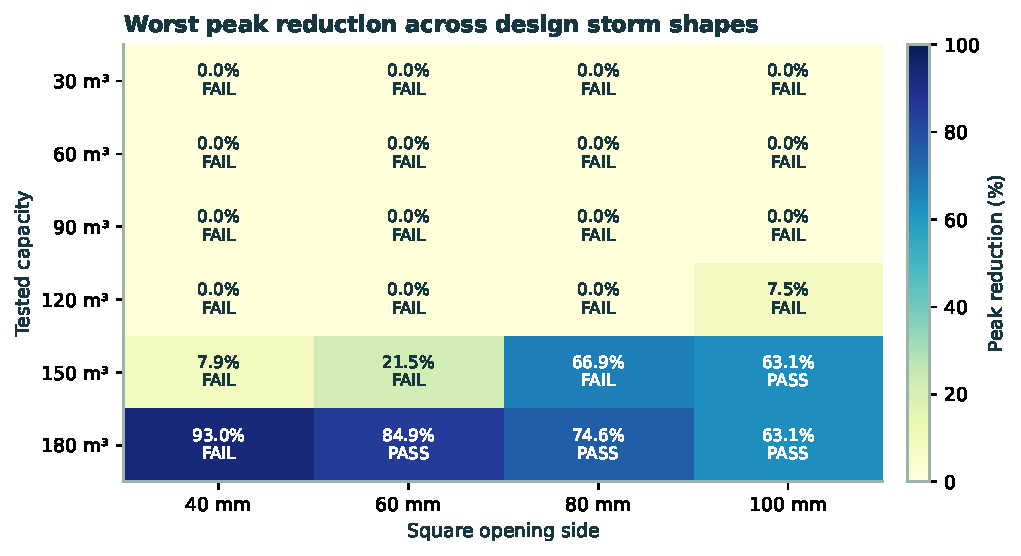
\includegraphics[width=0.93\linewidth]{figures/design_comparison.pdf}
\caption{Comparison of all 24 designs for the 50 mm storms. Cell values
show the smallest peak reduction across the three shapes. PASS requires all
three criteria for every shape. The full numerical table is provided in
Appendix~\ref{app:designs}.}\label{fig:comparison}
\end{figure}

\subsection{Hydrograph attenuation and timing}
Figure~\ref{fig:hydrographs} shows how the basin changes the response. Parking
runoff and direct rainfall create a relatively short inflow event; the basin
stores part of that input and releases it over a longer period. The
controlled-outlet peak is approximately 21--22 L/s for all three design
shapes, despite the wider range in baseline peaks.

\begin{figure}[htbp]
\centering
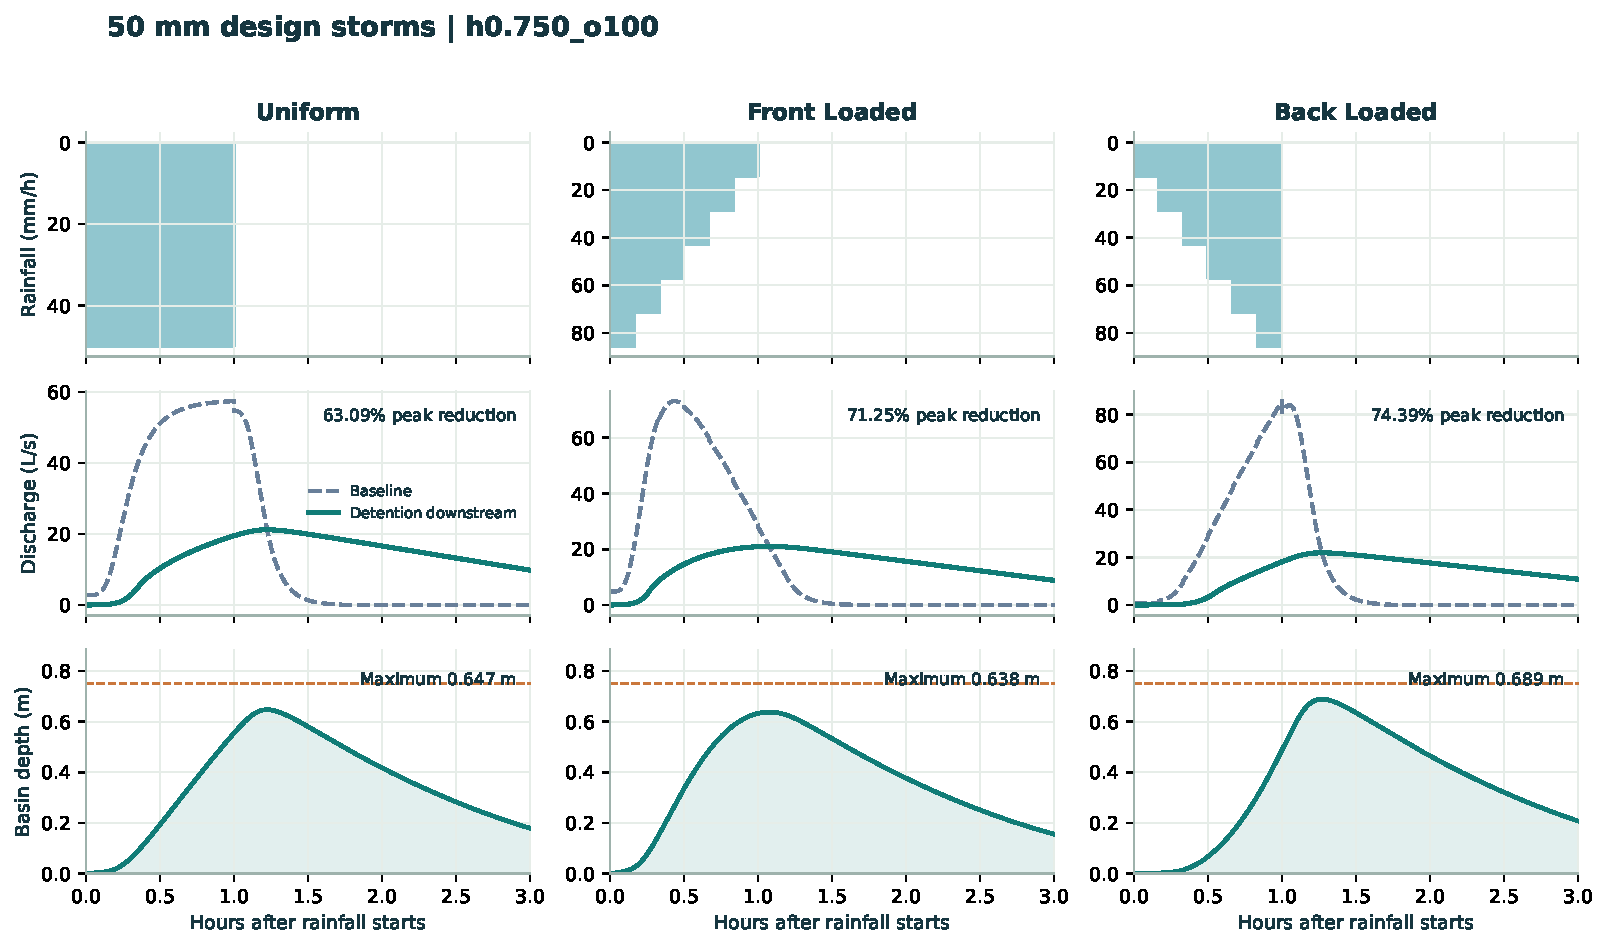
\includegraphics[width=\linewidth]{figures/design_hydrographs.pdf}
\caption{Rainfall, baseline and detained discharge, and basin depth for
the selected design under the 50 mm storms. The dashed depth line marks
nominal capacity. Curves show the first three hours; the drainage tail
continues beyond this window.}\label{fig:hydrographs}
\end{figure}

\begin{table}[H]
\centering\small
\caption{Time to peak from rainfall start for the selected design events.}
% Generated by generate_tables.py from source_data/.
\begin{tabular}{lrrr}
\toprule
Shape & Baseline peak (min) & Detained peak (min) & Peak delay (min) \\
\midrule
Uniform & 59.98 & 73.39 & 13.41 \\
Front-loaded & 26.23 & 64.58 & 38.34 \\
Back-loaded & 59.98 & 76.17 & 16.19 \\
\bottomrule
\end{tabular}

\source{Bundled \file{source_data/scenarios.csv}; interval-midpoint times.}
\end{table}
The detained peak occurs after rainfall ends in every design case. The
front-loaded case has the largest shift between baseline and detained peaks,
about 38.34 min. These timing changes describe the modeled comparison point;
the study does not route the discharge through a downstream channel network.

\subsection{Performance outside the design event}
The selected geometry is unchanged for the 25 and 100 mm tests.
Table~\ref{tab:all_events} presents all nine events together.
\begin{table}[H]
\centering\small
\caption{Selected-design results across all tested rainfall depths.}
\label{tab:all_events}
% Generated by generate_tables.py from source_data/.
\begin{tabular}{rlrrrrr}
\toprule
\shortstack{Rain\\(mm)} & Shape & \shortstack{Baseline\\(L/s)} & \shortstack{Detained\\(L/s)} & \shortstack{Reduction\\(\%)} & \shortstack{Overflow\\(m$^3$)} & \shortstack{Drawdown\\(h)} \\
\midrule
25 & Uniform & 27.77 & 12.77 & 54.02 & 0.000 & 6.39 \\
25 & Front-loaded & 32.68 & 12.52 & 61.69 & 0.000 & 6.23 \\
25 & Back-loaded & 40.90 & 13.45 & 67.12 & 0.000 & 6.53 \\
50 & Uniform & 57.48 & 21.22 & 63.09 & 0.000 & 7.65 \\
50 & Front-loaded & 73.19 & 21.04 & 71.25 & 0.000 & 7.51 \\
50 & Back-loaded & 85.67 & 21.94 & 74.39 & 0.000 & 7.81 \\
100 & Uniform & 116.19 & 116.19 & 0.00 & 162.526 & 7.97 \\
100 & Front-loaded & 154.83 & 149.86 & 3.21 & 163.580 & 7.87 \\
100 & Back-loaded & 173.96 & 173.96 & 0.00 & 173.330 & 8.02 \\
\bottomrule
\end{tabular}

\source{Bundled \file{source_data/scenarios.csv}. Numerically negligible
positive or negative reductions are displayed as 0.00\%.}
\end{table}

The 25 mm events produce no overflow and show peak reductions of
54.02--67.12\%. The 100 mm events fill the basin and generate
162.526--173.330 m$^3$ of overflow. Their downstream peak reductions are
approximately 0--3.21\%, because overflow carries much of the inflow past
the storage limit. Reporting the controlled outlet alone would conceal this
failure. The larger events are stress tests with no assigned return period.

\begin{figure}[htbp]
\centering
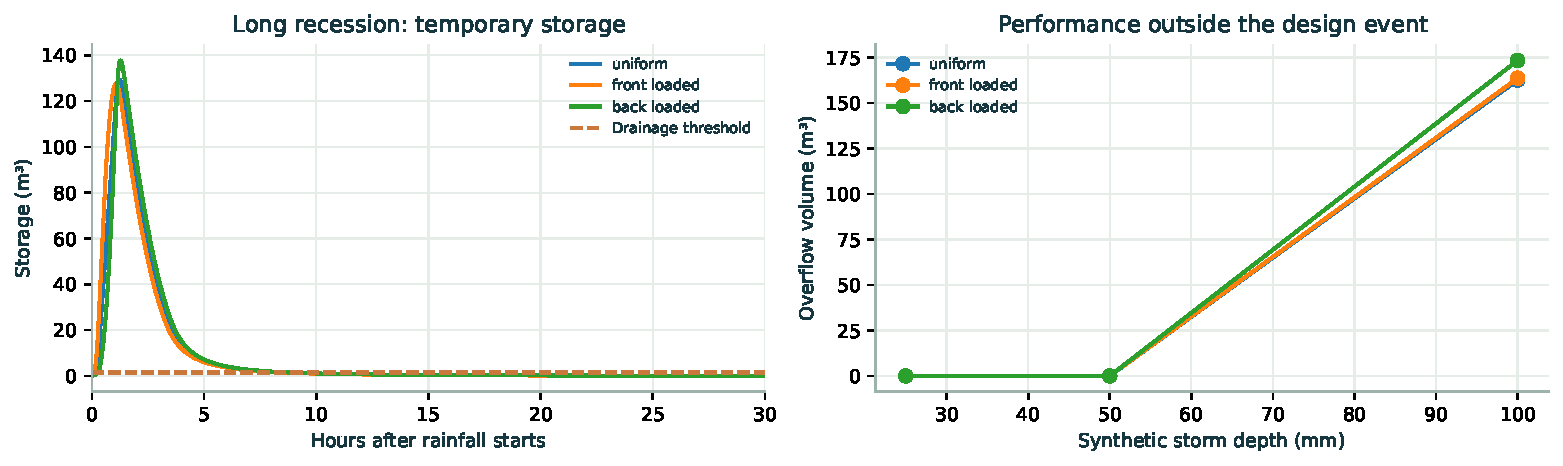
\includegraphics[width=\linewidth]{figures/drawdown_and_overflow.pdf}
\caption{Selected-design recession for the 50 mm storms and overflow
volume across rainfall depths. The drainage threshold is 1.50 m$^3$.
The overflow panel connects the three tested depths for visual comparison;
intermediate storm depths were not simulated in this study.}
\label{fig:tail}
\end{figure}

\subsection{Water budget and the meaning of detention}
With zero initial storage, basin infiltration, and evaporation, conservation
requires
\begin{equation}
 V_{\mathrm{input}}=V_{\mathrm{controlled}}+V_{\mathrm{overflow}}+
 V_{\mathrm{residual}}+\varepsilon_V,
 \label{eq:budget}
\end{equation}
where $\varepsilon_V$ is the numerical balance residual. The selected 50 mm
events use a 30 h horizon. Their small remaining volumes are shown explicitly.

\begin{table}[H]
\centering\small
\caption{Selected-design water budget at 30 h after rainfall starts.
``Discharged'' here denotes controlled outlet volume; overflow is separate.}
% Generated by generate_tables.py from source_data/.
\begin{tabular}{lrrrr}
\toprule
50 mm shape & Input (m$^3$) & Discharged (m$^3$) & Overflow (m$^3$) & Residual (m$^3$) \\
\midrule
Uniform & 187.103371 & 187.011722 & 0.000000 & 0.091649 \\
Front-loaded & 187.103371 & 187.012613 & 0.000000 & 0.090759 \\
Back-loaded & 187.103371 & 187.010723 & 0.000000 & 0.092649 \\
\bottomrule
\end{tabular}

\source{Bundled \file{source_data/scenarios.csv}. Display rounding can
produce a final-digit difference in the sum.}
\end{table}
Almost the entire inflow volume has been released by the horizon, with about
0.091--0.093 m$^3$ remaining. Detention changes when water is discharged; it
does not eliminate the 187.103 m$^3$ entering storage. Catchment losses in
the CN calculation occur before the basin and are the same in both
alternatives. They are not an additional volume-reduction benefit of the basin.

\FloatBarrier
\section{Verification and Numerical Reliability}\label{sec:verification}
\subsection{Boundary tests and independent calculations}
The numerical test suite contains 16 tests, all of which passed in the
recorded project run and passed again during preparation of this report.
They cover rainfall totals and partial blocks, zero and sub-abstraction
rainfall, CN~100, independent CN arithmetic, hydrograph volume and timing,
invalid inputs, empty storage, blocked outlets, insufficient capacity,
outlet quadrature, deep-orifice comparison, monotonicity, shallow drainage,
final drainage crossing, and stepwise continuity.

For the outlet rating, independent numerical quadrature agrees with the
integrated formula to a maximum absolute difference of approximately
$2.08\times10^{-17}$ m$^3$/s in the saved checks. This tests the implementation
of the idealized equation; it does not calibrate the physical coefficient.

When the basin is shallow enough that $h<a$ and no inflow remains, define
$k=(2/3)C_d a\sqrt{2g}$. Then the model reduces to
$A_b\,dh/dt=-kh^{3/2}$, with analytical solution
\begin{equation}
 h(t)=\left[h_0^{-1/2}+\frac{k}{2A_b}t\right]^{-2}.
 \label{eq:analytical}
\end{equation}
For the saved test with $A_b=200$ m$^2$, $h_0=0.02$ m, $a=0.06$ m,
and duration 1 h, the exact final depth is 0.015394949 m. Relative numerical
error decreases from 0.04004\% at 30 s to 0.02004\% at 15 s and
0.01003\% at 7.5 s. This is consistent with the expected convergence of
the chosen first-order time integration.

The companion workbook independently implements the runoff equations,
a blocked-storage fixture, and 45 bisection iterations for a controlled-outlet
step. The saved artifact audit reports that all 356 workbook formulas were
re-evaluated and their cached values checked. These checks are automated;
they do not claim a manual Excel session.

\subsection{Time-step refinement}
The full 216-case grid was repeated at 30, 15, 7.5, 3.75, and 1.875 s.
For a metric $M$, the reported relative change is
\begin{equation}
 \delta_M=\frac{|M_{\mathrm{coarse}}-M_{\mathrm{fine}}|}
 {\max(|M_{\mathrm{fine}}|,10^{-12})}.
 \label{eq:convergence}
\end{equation}
Table~\ref{tab:convergence} gives the largest changes across the entire
grid for each successive pair. Different maxima may occur in different cases.

\begin{table}[H]
\centering\small
\caption{Grid-wide time-step convergence. Peak and storage changes are
percentages; overflow and drawdown changes are absolute.}\label{tab:convergence}
% Generated by generate_tables.py from source_data/.
\begin{tabular}{rrrrr}
\toprule
Steps (s) & \shortstack{Peak change\\(\%)} & \shortstack{Storage change\\(\%)} & \shortstack{Overflow change\\(m$^3$)} & \shortstack{Drawdown change\\(s)} \\
\midrule
30 / 15 & 9.0505 & 0.2712 & 0.437721 & 67.253 \\
15 / 7.5 & 3.5158 & 0.1367 & 0.217996 & 33.573 \\
7.5 / 3.75 & 3.4323 & 0.0686 & 0.109471 & 16.772 \\
3.75 / 1.875 & 0.9078 & 0.0342 & 0.054714 & 8.389 \\
\bottomrule
\end{tabular}

\source{Bundled \file{source_data/convergence.csv}.}
\end{table}

The final maximum downstream-peak change is 0.9078\%; maximum-storage change
is 0.0342\%. Baseline-peak change is at most 0.0472\%. All are below 1\%.
The winner, event pass/fail decisions, and overflow classifications are stable
at the final pair. Maximum final overflow-onset movement is 1.875 s;
drawdown movement is 8.389 s. Coarser resolutions were insufficient for some
overflowing alternatives, even though the design decision was already stable.

These results quantify discretization sensitivity for the stated model.
They do not establish an error bound relative to measured site behavior.

\subsection{Water-balance closure and reproducibility}
The largest recorded absolute residuals across nominal and sensitivity cases
are $1.42\times10^{-14}$ m$^3$ for runoff generation,
$2.84\times10^{-14}$ m$^3$ for hydrograph transformation, and
$1.00\times10^{-9}$ m$^3$ for storage routing. The largest relative routing
residual is $5.36\times10^{-12}$, well below the configured 0.1\% relative
tolerance with a $10^{-8}$ m$^3$ absolute allowance.

The existing reproducibility record reports a complete rerun with exact
agreement in every compared non-runtime field of the 216-row scenario table,
the nine-row baseline table, and the 27-row sensitivity table, as well as an
identical selection. During preparation of this report, current project source
hashes were checked against that run's manifest and all matched. The new
report uses those saved results; it does not present a newly executed full
scenario sweep as additional evidence.\cite{project_data}

\section{Sensitivity Results}\label{sec:sensitivity}
Table~\ref{tab:sensitivity} summarizes each one-at-a-time parameter variation
across the three design storm shapes. The geometry remains fixed at 150 m$^3$
with the 100 mm opening. Each column reports its own worst case, so the
minimum peak reduction, maximum overflow, and maximum drawdown in a row
need not occur in the same shape.

\begin{table}[H]
\centering\small
\caption{Selected-design sensitivity for the 50 mm events. Nominal parameter
values repeat intentionally in each group.}\label{tab:sensitivity}
% Generated by generate_tables.py from source_data/.
\begin{tabular}{lrrrrl}
\toprule
Parameter & Value & \shortstack{Min. reduction\\(\%)} & \shortstack{Max. overflow\\(m$^3$)} & \shortstack{Max. drawdown\\(h)} & All shapes \\
\midrule
Curve number & 95 & 64.37 & 0.000 & 7.52 & Pass \\
Curve number & 98 & 63.09 & 0.000 & 7.81 & Pass \\
Curve number & 100 & 47.25 & 2.841 & 7.95 & \textbf{Fail} \\
Lag (min) & 5 & 62.47 & 0.000 & 7.71 & Pass \\
Lag (min) & 10 & 63.09 & 0.000 & 7.81 & Pass \\
Lag (min) & 15 & 63.40 & 0.000 & 7.90 & Pass \\
$C_d$ & 0.5 & 69.16 & 0.000 & 9.72 & Pass \\
$C_d$ & 0.62 & 63.09 & 0.000 & 7.81 & Pass \\
$C_d$ & 0.75 & 57.01 & 0.000 & 6.42 & Pass \\
\bottomrule
\end{tabular}

\source{Bundled \file{source_data/sensitivity.csv}.}
\end{table}

\textbf{Curve number is the tested assumption that changes feasibility.}
CN~95 and CN~98 pass all three shapes, while CN~100 fails for the back-loaded
storm. That case produces 2.841 m$^3$ of overflow and only 47.25\% peak
reduction. With CN~100, all 50 mm of parking rainfall becomes modeled runoff,
so total input is 210 m$^3$, about 22.90 m$^3$ greater than the nominal input.
The routed outcome demonstrates that the selected design is not robust to
every runoff assumption tested.

Changing lag from 5 to 15 min preserves feasibility throughout this
one-at-a-time experiment. Worst-case peak reductions stay between 62.47\%
and 63.40\%, and drawdown remains under 7.90 h. This comparatively small
response applies to the tested range and fixed storm duration.

The discharge coefficient shows the expected storage--release tradeoff.
Reducing $C_d$ to 0.50 improves worst-case peak attenuation to 69.16\% but
extends maximum drawdown to 9.72 h. Increasing it to 0.75 shortens drawdown
to 6.42 h while reducing worst-case attenuation to 57.01\%. Both still meet
the nominal objectives, and neither produces overflow in these scenarios.

The experiments establish where the selected design is sensitive within
the supplied parameter grid. They do not provide a probability of failure:
the parameter values are illustrative, only one parameter changes at a time,
and no measured distribution or joint uncertainty model is available.

\section{Engineering Discussion and Conclusions}\label{sec:discussion}
\subsection{What the design comparison establishes}
The project meets its central analytical goal: it identifies a reproducible
minimum among the \emph{tested} feasible capacities and explains the mechanism
behind that choice. The 150 m$^3$/100 mm configuration balances enough
temporary storage with enough controlled release to avoid overflow across
the nominal 50 mm storm shapes. Its smallest peak reduction exceeds the
target by 13.09 percentage points, and its longest drawdown is comfortably
below 24 h under the adopted assumptions.

The storage value is not a continuously optimized minimum. Candidate
capacities are separated by 30 m$^3$, and openings are sampled at 20 mm
increments. A capacity between the tested values, or a different outlet
geometry, may change the minimum. The current result should therefore be
stated as the smallest \emph{tested passing} design, not the unique global
optimum or a least-cost design.

The comparison also requires care when interpreting drainage. At the same
100 mm opening, 180 m$^3$ of capacity gives the same nominal 50 mm hydrograph
as 150 m$^3$, because neither capacity binds the water level. Its reported
drawdown is shorter because 1\% of 180 m$^3$ is 1.80 m$^3$, a higher threshold
than 1.50 m$^3$. That difference does not demonstrate a faster physical
release rate. Capacity-dependent recovery criteria should be kept visible
when alternatives are compared.

\subsection{Limitations and appropriate next engineering steps}
The most important limitation is the gap between a verified numerical
implementation and a validated site model. No field survey, soil study,
rainfall-runoff observations, or calibrated outlet rating was provided.
The synthetic storms are not assigned a frequency, and the acceptance
criteria are not a regulatory compliance assessment. The constant-area basin
and free-discharge opening omit grading, tailwater, conveyance, freeboard,
and overflow-path hydraulics.

The saved results identify two concrete priorities for further work. First,
the CN~100 back-loaded failure warrants refining the design under more
conservative runoff assumptions before asserting a robust recommendation.
Second, the substantial 100 mm overflow shows the need to evaluate an
engineered exceedance route if the concept is applied to an actual site.
Numerical overflow volumes alone do not locate or size that route.

A subsequent design phase would replace the assumed site geometry and
hydrologic inputs with appropriate local information, verify the design
storm basis, and assess a realistic stage--storage relationship and outlet
system. It could then refine the capacity and opening grid, test combined
uncertainty, include tailwater and partial blockage, and examine closely
spaced storms with residual initial storage. Cost and maintainability would
be additional decision criteria in that phase. These activities are proposed
extensions; they are not completed results of this project.

\subsection{Final conclusions}
\begin{enumerate}
\item A 150 m$^3$ basin with a 100 $\times$ 100 mm square opening is the
smallest tested configuration meeting all three objectives for every nominal
50 mm storm shape.
\item The selected design reduces peak flow by 63.09--74.39\%, avoids
overflow, and reaches the stated drainage threshold within 7.81 h after
rainfall ends. Its maximum simulated design-event depth is 0.6888 m.
\item The selection depends on the stated conditions. All 100 mm storm
shapes overflow substantially, and the CN~100 back-loaded 50 mm case fails
the overflow and peak criteria.
\item Numerical tests, independent calculations, water balance, full-grid
refinement, and recorded reproducibility support the computational findings.
They establish numerical reliability within the conceptual model's scope.
\item The modeled benefit is temporary storage and peak attenuation.
With zero basin infiltration and evaporation, the incoming runoff remains
accounted for as controlled discharge, overflow, or residual storage.
\end{enumerate}

\clearpage
\appendix
\section{Complete Nominal Design Comparison}\label{app:designs}
Every row summarizes the three 50 mm storm shapes for one capacity--opening
combination. Minimum reduction, maximum overflow, and maximum drawdown
are taken separately across shapes. Passing requires all criteria in all
three events. Opening dimensions are square side lengths.

\begin{table}[H]
\centering\small
\caption{All 24 tested designs, final time step 1.875 s.}
% Generated by generate_tables.py from source_data/.
\begin{tabular}{rrrrrrl}
\toprule
\shortstack{Capacity\\(m$^3$)} & \shortstack{Depth\\(m)} & \shortstack{Opening\\(mm)} & \shortstack{Min. reduction\\(\%)} & \shortstack{Max. overflow\\(m$^3$)} & \shortstack{Max. drawdown\\(h)} & Result \\
\midrule
30 & 0.15 & 40 & 0.00 & 150.518 & 37.81 & Fail \\
30 & 0.15 & 60 & 0.00 & 143.966 & 24.52 & Fail \\
30 & 0.15 & 80 & 0.00 & 136.195 & 18.26 & Fail \\
30 & 0.15 & 100 & 0.00 & 127.753 & 14.61 & Fail \\
60 & 0.30 & 40 & 0.00 & 118.358 & 30.57 & Fail \\
60 & 0.30 & 60 & 0.00 & 109.490 & 18.78 & Fail \\
60 & 0.30 & 80 & 0.00 & 98.708 & 13.61 & Fail \\
60 & 0.30 & 100 & 0.00 & 86.586 & 10.72 & Fail \\
90 & 0.45 & 40 & 0.00 & 87.082 & 28.67 & Fail \\
90 & 0.45 & 60 & 0.00 & 76.995 & 16.81 & Fail \\
90 & 0.45 & 80 & 0.00 & 64.800 & 11.87 & Fail \\
90 & 0.45 & 100 & 0.00 & 51.219 & 9.19 & Fail \\
120 & 0.60 & 40 & 0.00 & 56.237 & 28.30 & Fail \\
120 & 0.60 & 60 & 0.00 & 45.442 & 15.98 & Fail \\
120 & 0.60 & 80 & 0.00 & 32.549 & 11.02 & Fail \\
120 & 0.60 & 100 & 7.49 & 18.459 & 8.41 & Fail \\
150 & 0.75 & 40 & 7.87 & 25.671 & 28.57 & Fail \\
150 & 0.75 & 60 & 21.46 & 14.501 & 15.64 & Fail \\
150 & 0.75 & 80 & 66.92 & 1.441 & 10.57 & Fail \\
150 & 0.75 & 100 & 63.09 & 0.000 & 7.81 & \textbf{Selected} \\
180 & 0.90 & 40 & 92.96 & 0.000 & 28.84 & Fail \\
180 & 0.90 & 60 & 84.87 & 0.000 & 15.08 & Pass \\
180 & 0.90 & 80 & 74.63 & 0.000 & 9.84 & Pass \\
180 & 0.90 & 100 & 63.09 & 0.000 & 7.20 & Pass \\
\bottomrule
\end{tabular}

\source{Bundled \file{source_data/design_selection.csv}.}
\end{table}

Small values near zero peak reduction are rounded to zero for readability.
No candidate below 150 m$^3$ passes. The selected design is the sole passing
150 m$^3$ alternative, so the secondary tie rules do not change the winner.

\clearpage
\section{Reproducibility, Deliverables, and Contribution Record}\label{app:reproduction}
\subsection{Reproducing the numerical study}
The recorded run used Python 3.14.3 on macOS arm64. Key recorded package
versions were NumPy 2.4.3, pandas 2.3.3, SciPy 1.17.1, Matplotlib 3.10.9,
Plotly 6.7.0, openpyxl 3.1.5, XlsxWriter 3.2.9, and PyMuPDF 1.28.0.
The project includes local input files and does not make network requests
during a study run. The root \file{requirements.txt} lists dependency
requirements; pdfLaTeX is used for the original report build.

From the project root on the documented machine, the complete original
workflow can be run with:
\begin{lstlisting}
conda run -n psrc python run_project.py
\end{lstlisting}
The default command regenerates the original project outputs. To preserve
the saved study while running a changed configuration, use a separate output
directory, for example:
\begin{lstlisting}
conda run -n psrc python run_project.py \
  --config inputs/my_experiment.json \
  --output-dir experiments/my_experiment
\end{lstlisting}
The alternative configuration must first be created by copying and editing
the supplied input file. This command illustrates reproduction and extension;
it does not imply that such an additional experiment was performed for this
report. Model tests can be run independently with
\file{python -m unittest discover -s tests -v}.

The recorded study stage took 301.60 s, and the complete recorded command
took 314.25 s. Median final-resolution case time was 0.3663 s, and the
slowest case took 1.1556 s. Recorded peak Python-process memory was
408.52 MiB, excluding child processes. These are measurements from the saved
run on that machine, rather than general performance guarantees or timing
for this expanded report build.

\subsection{Project deliverables and this report package}
\begin{table}[H]
\centering\small
\caption{Deliverables produced by the project and their intended uses.}
\begin{tabularx}{\linewidth}{>{\raggedright\arraybackslash}p{0.43\linewidth}Y}
\toprule
File or directory at the project root & Purpose \\
\midrule
\file{stormwater_dashboard.html} & Offline exploration of all 216 cases and
the matching baselines. \\
\file{stormwater_calculations.xlsx} & Scenario tables, formula-based
independent checks, and charts. \\
\file{site_plan.pdf}, \file{site_plan.svg}, \file{site_plan.dxf} & Conceptual
plan and section, including editable drawing formats. \\
\file{results/} & Saved metrics, full time-series arrays, source snapshots,
manifest, convergence, and verification records. \\
\file{engineering_report.tex} and PDF & Original brief generated report. \\
\file{FINDINGS.md}, \file{LEARNING_GUIDE.md} & Findings and worked learning
material. \\
\file{manasi_project_report/} & This expanded engineering report, editable
LaTeX, PDF, figure assets, numerical tables, and evidence snapshots. \\
\bottomrule
\end{tabularx}
\end{table}

This report folder is self-contained for LaTeX compilation. Run
\file{sh build_report.sh} inside it to rebuild the PDF. The included
\file{generate_tables.py} uses only Python's standard library and rebuilds
tables from the bundled evidence snapshot. Rebuilding tables does not rerun
the engineering model or revise the narrative automatically. If new model
results are adopted later, the source snapshot, tables, figures, and written
interpretation should be updated together.

\subsection{Evidence and actual contributions}
The supplied project plan defined the technical scope. Codex implemented
and executed the numerical study, developed the automated checks, and created
the workbook, dashboard, figures, drawings, and documentation. This expanded
report was prepared from the saved project evidence with Codex assistance.

The project contribution record does not verify Manasi's personal coding,
manual Excel calculations, CAD edits, or independent interpretation.
Those activities remain for her to record in \file{MANASI_REVIEW.md}; the
report does not sign or complete that review on her behalf. This distinction
preserves an accurate record of the completed technical work and the
remaining individual learning activities.\cite{contributions}

The new package's \file{source_data/report_provenance.json} identifies its
copied evidence and source-hash checks. The original artifact audit and
reproducibility records refer to the original project deliverables. Compilation
and layout checks for this expanded report are recorded separately under
\file{build/}.

\clearpage
\phantomsection
\addcontentsline{toc}{section}{References}
\begin{thebibliography}{99}
\small\raggedright
\bibitem{project_plan}
\emph{Parking-Lot Stormwater Detention: Simulation and Design Comparison}.
Local project specification, \file{PROJECT_PLAN.md}, completed-study status
dated September 8, 2026. Read together with \file{README.md} and
\file{FINDINGS.md} in the project root.

\bibitem{cn}
U.S. Army Corps of Engineers, Hydrologic Engineering Center.
\href{https://www.hec.usace.army.mil/confluence/hmsdocs/hmstrm/canopy-surface-infiltration-and-runoff-volume/infiltration/scs-curve-number-loss-model}
{\emph{SCS Curve Number Loss Model}}, HEC-HMS Technical Reference Manual.
Accessed September 8, 2026. Basis for cumulative event runoff equations and
incremental excess rainfall.

\bibitem{uh}
U.S. Army Corps of Engineers, Hydrologic Engineering Center.
\href{https://www.hec.usace.army.mil/confluence/hmsdocs/hmstrm/transform/scs-unit-hydrograph-model}
{\emph{SCS Unit Hydrograph Model}}, HEC-HMS Technical Reference Manual.
Accessed September 8, 2026. Basis for dimensionless hydrograph interpretation
and $T_p=t_{\mathrm{lag}}+\Delta t/2$.

\bibitem{ordinates}
Texas Department of Transportation.
\href{https://www.txdot.gov/manuals/des/hyd/chapter-4--hydrology/section-13--hydrograph-method/nrcs-dimensionless-unit-hydrograph.html}
{\emph{NRCS Dimensionless Unit Hydrograph}}, Hydraulic Design Manual,
Chapter 4, Section 13, Table 4-29. Accessed September 8, 2026.
Source of the 33 reference ordinate pairs stored with the project.

\bibitem{routing}
U.S. Army Corps of Engineers, Hydrologic Engineering Center.
\href{https://www.hec.usace.army.mil/confluence/hmsdocs/hmstrm/reservoir-modeling/reservoir-modeling-concepts-and-equations}
{\emph{Reservoir Modeling Concepts and Equations}}, HEC-HMS Technical
Reference Manual. Accessed September 8, 2026. Background for level-pool
continuity and stage--storage--outflow relationships; the project implements
backward Euler rather than the manual's trapezoidal routing scheme.

\bibitem{outlet}
U.S. Army Corps of Engineers, Hydrologic Engineering Center.
\href{https://www.hec.usace.army.mil/confluence/hmsdocs/hmsum/latest/reservoir-elements/outflow-structures-routing}
{\emph{Outflow Structures Routing}}, HEC-HMS User's Manual.
Accessed September 8, 2026. Background on outlet regimes and limitations;
the integrated square-opening rating used here is a project idealization.

\bibitem{method_selection}
Texas Department of Transportation.
\href{https://www.txdot.gov/manuals/des/hyd/chapter-4--hydrology/section-7--selection-of-the-appropriate-method-for.html}
{\emph{Selection of the Appropriate Method for Calculating Runoff}},
Hydraulic Design Manual, Chapter 4, Section 7. Accessed September 8, 2026.
Background for using a hydrograph when evaluating storage.

\bibitem{project_data}
\emph{Manasi project numerical results and verification evidence}.
Saved run completed September 8, 2026, 21:44:16 UTC.
\file{results/scenarios.csv}, \file{results/baselines.csv},
\file{results/design_selection.csv}, \file{results/selection.json},
\file{results/convergence.csv}, \file{results/sensitivity.csv},
\file{results/independent_checks.json}, \file{results/run_manifest.json},
\file{results/artifact_audit.json}, and
\file{results/reproducibility_check.json}. Copies supporting this report
are bundled in \file{source_data/}.

\bibitem{contributions}
\emph{Contribution and Assistance Record} and \emph{Manasi's Personal Review}.
Local project files \file{CONTRIBUTIONS.md} and \file{MANASI_REVIEW.md},
reviewed for this report on September 8, 2026.
\end{thebibliography}
\end{document}
